\chapter{Ближче до справи} 
\label{chapter:first}

Оскільки тут описувати по суті нічого, адже автори щиро вірять у казочку, що усі грали ці ігри, перейдемо відразу до технічних деталей.

\section{Підключення матриці}

Розпіновка світлодіодної матриці показана на \ref{matrix}
\begin{figure}[h]
\center{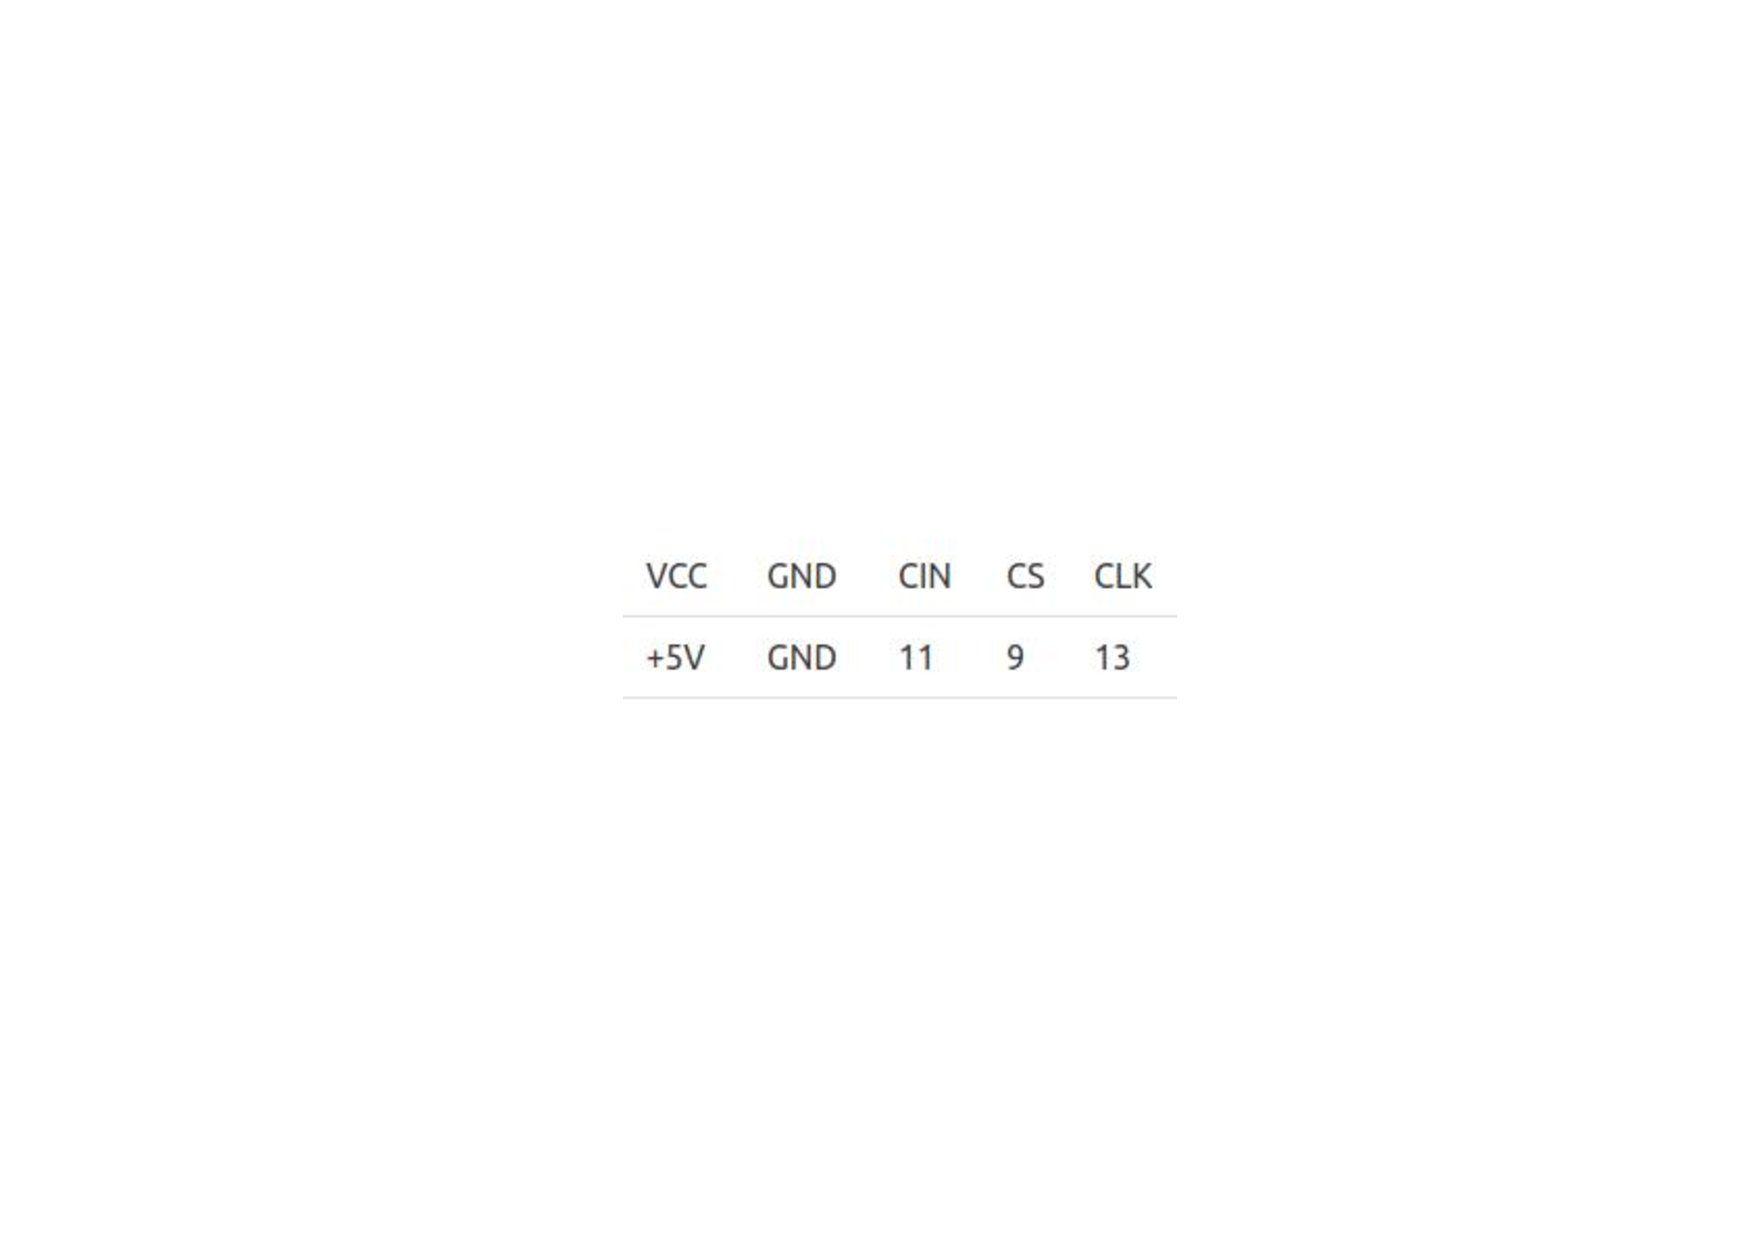
\includegraphics[width=0.9\linewidth]{matrix.pdf}}
\caption{Розпіновка світлодіодної матриці.}
\label{matrix}
\end{figure}

\section{Змійка}

Відео гри одного з авторів у отриману змійку знаходиться у нашій папці на гітхабі.

Програмний код: 
\lstinputlisting[language=c++]{snake.ino}


\section{Тетріс}

Відео гри одного з авторів у отриманий тетріс знаходиться у нашій папці на гітхабі.

Програмний код: 
\lstinputlisting[language=c++]{tetris.ino}
